\chapter{Analiza wyników}
\label{cha:analiza_wynikow}

Ostateczny model klasyfikatora po dobraniu odpowiedniej architektury i dostrojeniu parametrów został przetrenowany przez 36 epok, a ostatnia poprawa wartości funkcji błedu nastąpiła w 29 epoce. Przebieg procesu uczenia został przedstawiony na Rys. \ref{fig:trening_model_4}. Krzywa walidacji prawie w każdym punkcie nadąża za krzywą uczenia, co oznacza stabilność algorytmu. Wartość skuteczności modelu na zbiorze testowym wynosi 85\% (\ref{tab:acc}).

\begin{figure}[h!]
	\centering
	\centering
		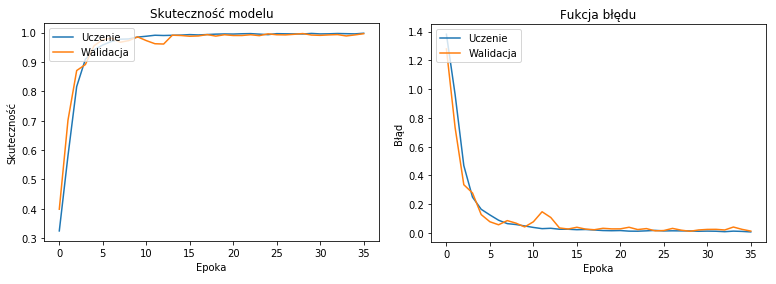
\includegraphics[scale=0.5]{trening_model_4}	
	\caption{Zależność skuteczności i błędu od epoki w procesie uczenia opracowanego klasyfikatora.}\label{fig:trening_model_4}
\end{figure}

\begin{table}[h!]
\centering
\caption[Short Heading]{Skuteczność opracowanego klasyfikatora.}
\label{tab:acc}
\begin{tabular}{|c|c|c|c|}
\hline
\textbf{typ zbioru}           & \textbf{treningowy} & \textbf{walidacyjny} & \textbf{testowy} \\ \hline
\textbf{skuteczność {[}\%{]}} & 99                  & 99                   & 85               \\ \hline
\end{tabular}
\end{table}

{\parindent0pt
Do klasyfikacji używany jest model uczony przez 29 epok. Dane wejściowe są w obrazami RGB o wymiarach 120x160, przeskalowanymi do zakresu wartości pikseli 0-1. Ramki podzielone są na porcje po 32 obrazy, co daje 248 iteracji w każdej epoce uczenia zgodnie ze wzorem (\ref{equ:iter_num_trening}). Testowanie odbywa się w 62 iteracjach, zgodnie ze wzorem (\ref{equ:iter_num_test}). Takie podejście pozwala na przejście wszystkich danych przez system w każdej epoce, zarówno podczas uczenia, jak i testowania.

\begin{equation}
i = \floor*{\frac{x}{b}} = \floor*{\frac{7965}{32}} = 248
\label{equ:iter_num_trening}
\end{equation}
gdzie,
\begin{eqwhere}[2cm]
	\item[$i$] ilość iteracji w jednej epoce treningu,
	\item[$x$] ilość ramek treningowych,
	\item[$b$] ilość ramek w porcji.
\end{eqwhere}

\begin{equation}
j = \floor*{\frac{y}{b}} = \floor*{\frac{1992}{32}} = 62
\label{equ:iter_num_test}
\end{equation}
gdzie,
\begin{eqwhere}[2cm]
	\item[$j$] ilość iteracji teście,
	\item[$y$] ilość ramek testowych,
	\item[$b$] ilość ramek w porcji.
\end{eqwhere}

Na podstawie ogólnej macierzy pomyłek (\ref{tab:general_conf_matrix}) można wyprowadzić macierze dla każdej klasy osobno i wyprowadzić parametry pozwalające na dokładniejszą analizę jakości klasyfikacji.

\begin{table}[h!]
\centering
\caption[Short Heading]{Macierz pomyłek zbioru testowego opracowanego klasyfikatora.}
\label{tab:general_conf_matrix}
\begin{tabular}{|c|c|c|c|c|c|}
\hline
\textbf{}                           & \multicolumn{5}{c|}{\textbf{predykcja}} \\ \hline
{\multirow{5}{*}{\rotatebox[origin=c]{90}{\textbf{klasa}}}} &         & E       & L        & M      & N       \\ \cline{2-6} 
                                    & E       & 141       & 144      & 141     & 197      \\ \cline{2-6} 
                                    & L       & 134       & 149      & 130      & 207      \\ \cline{2-6} 
                                    & M       & 145       & 128      & 141      & 206      \\ \cline{2-6} 
                                    & N       & 140       & 137      & 140      & 207       \\ \hline
\end{tabular}
\end{table}

\begin{table}[h!]
\centering
\caption[Short Heading]{Parametry mierzące jakość klasyfikacji na zbiorze testowym opracowanego klasyfikatora.}
\label{tab:kaggle_1_params_val_1}
\begin{tabular}{|c|c|c|c|c|}
\hline
\textbf{Parametr}                               & \textbf{Precyzja} & \textbf{Czułość} & \textbf{Miara F1} & \textbf{Ilość próbek} \\ \hline
\textbf{klasa eozynofil (E)} & 0.25   & 0.23   & 0.24  & 623  \\ \hline
\textbf{klasa limfocyt (L)} & 0.27  & 0.24 & 0.25  & 620  \\ \hline
\textbf{klasa monocyt (M)} & 0.26   & 0.23    & 0.24  & 620  \\ \hline
\textbf{klasa neutrofil (N)} & 0.25   & 0.33   & 0.29  & 624  \\ \hline
\end{tabular}
\end{table}
}